\cotefile{156-7}
\scanpage{101}
\handwritten{
\mspage{100}
% Two vertical emphasis strokes beside the corollary.
\margin{$\Vert$\quad ?}
\uline{Corollaire} $\forall Z\in\unsure{\mathcal M|M}$ tel que \inserted{$\forall X'\in\widetilde F^{\circ}$, on ait} $Z\parallel\deleted{X}\operatorname{omb}(X')^{\circ}$ et \deleted{\unsure{Alors soit}} $Z\parallel\unsure{\operatorname{omb}|\operatorname{int}}(X)^{\circ}$.

\inserted{\uline{Par \unsure{At L2}}} On est ramené au cas où $Z=x\in\unsure{\mathcal L|L}$.

Je rappelle que $F\preccurlyeq X$ signifie $F\ll X$ et $\operatorname{supp}. F=\mathrm{s}\text{-}\unsure{\mathscr W|W}X$. Si on a une fonction $\deleted{\unsure{\mathrm{s}\text{-}\mathscr W X}}\inserted{X\longrightarrow |X|}$ à valeurs dans un \unsure{ens.} $P$ (cf. p.\,80, condition $\mathrm{S}\text{-}\mathscr W_{\unsure{\phi|p}}1$ -- \unsure{ou|on} un $\mathrm{s}\text{-}\mathscr W$-\unsure{inv} par $\mathrm{S}\text{-}\mathscr W_{\phi}2$) alors pour $F\ll X$, la condition $F\preccurlyeq X$ signifie simplement que $\deleted{\unsure{\partial}}|F|=|X|$. Je dis que \deleted{\unsure{les}}
% margin note written sideways / slanted
\margin{On doit $\mathrm{s}\text{-}\mathscr W$ \unsure{non} \unsure{coW} $\unsure{K\longleftrightarrow X|K\ll X}$.}
\[
\left\{\begin{aligned}
\text{\textcircled{a}}\quad \deleted{\unsure{\operatorname{supp}}}\quad |X^{\circ}|&=|X|\setminus|\partial X|,\quad\text{et que}\\
\text{\textcircled{b}}\quad \deleted{\unsure{\widetilde F\preccurlyeq F}}\quad \widetilde F^{\circ}&=\{X'\in\widetilde F\mid |X'^{\circ}|\subset|X^{\circ}|\}\\
&=\{X'\in\widetilde F\mid |X'^{\circ}|\cap|X^{\circ}|\ne\varnothing\}
\end{aligned}\right.
\]
\margin{$\unsure{B}$}

Comme $X^{\circ}\parallel\partial X$, \deleted{\unsure{on a}} et $X^{\circ}\subset\deleted{X}\inserted{\mathrm{s}\text{-}\mathscr W X}$, on a $|X^{\circ}|\subset|X|=|\mathrm{s}\text{-}\mathscr W X|$, et $|X^{\circ}|\cap|\partial X|=\varnothing$, donc
\[
\unsure{=|\Rightarrow}\quad |X^{\circ}|\subset|X|\setminus|\partial X|
\]
% Two horizontal separator strokes above the reused typescript.
\figure{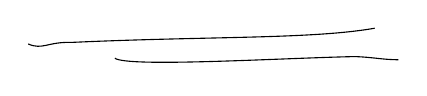
\begin{tikzpicture}[x=1cm,y=1cm]
\draw (0,0.20) .. controls (0.18,0.12) and (0.25,0.23) .. (0.55,0.22) .. controls (2.3,0.30) and (3.6,0.26) .. (4.4,0.40);
\draw (1.10,0.02) .. controls (1.25,-0.10) and (3.2,0.02) .. (4.15,0.04) .. controls (4.4,0.03) and (4.5,0.00) .. (4.7,0.00);
\end{tikzpicture}}
}
% Reused typescript below is upside down relative to the manuscript.
% Three diagonal cancellation strokes pass through the whole typed block.
\mspage{\deleted{A 6}}
\deleted{de "mot de la fin", pas de "conclusions" dans Récoltes et Semailles; pas plus qu'il n'y en a dans ma vie, ou dans la tienne. Il y a un vin, vieilli pendant une vie dans les fûts de mon être. Le dernier verre que tu boiras ne sera pas meilleur que le premier ou que le centième . Ils sont tous "le même", et ils sont tous différents. Et si le premier verre est gâté, tout le tonneau l'est ; autant alors boire de la bonne eau (s'il s'en trouve), plutôt que du mauvais vin.}

\deleted{Mais un bon vin ne se boit pas à la va-vite, ni au pied levé.}
